%============================================================
%  TTM Challenge – Group 42  |  IIT  |  CS671
%  Overleaf LaTeX Beamer Presentation
%  Compile with: pdflatex → biber (optional) → pdflatex × 2
%  All results are from actual evaluation (fusion/results/)
% ============================================================
\documentclass[aspectratio=169, 10pt]{beamer}

% ── Packages ─────────────────────────────────────────────────────────────────
\usepackage[T1]{fontenc}
\usepackage[utf8]{inputenc}
\usepackage{lmodern}
\usepackage{tikz}
\usepackage[x11names,table]{xcolor}
\usetikzlibrary{arrows.meta, positioning, shapes.geometric, fit, backgrounds, calc}
\usepackage{pgfplots}
\usepackage{pgffor}
\pgfplotsset{compat=1.18}
\usepackage{booktabs}
\usepackage{multirow}
\usepackage{array}
\usepackage{colortbl}
\usepackage{xcolor}
\usepackage{amsmath, amssymb}
\usepackage{etoolbox}
\usepackage{mathtools}
\usepackage{graphicx}
\usepackage{tcolorbox}
\tcbuselibrary{skins, breakable}
\usepackage{enumitem}
\usepackage{microtype}

% ── Color Definitions ────────────────────────────────────────────────────────
\definecolor{NavyBlue}{RGB}{13,42,74}
\definecolor{AccBlue}{RGB}{21,101,192}
\definecolor{AccTeal}{RGB}{0,137,123}
\definecolor{AccOrange}{RGB}{230,81,0}
\definecolor{AccPurple}{RGB}{106,27,154}
\definecolor{AccRed}{RGB}{198,40,40}
\definecolor{AccGreen}{RGB}{46,125,50}
\definecolor{LightBg}{RGB}{247,249,252}
\definecolor{CardBlue}{RGB}{232,240,254}
\definecolor{CardTeal}{RGB}{224,242,241}
\definecolor{CardOrange}{RGB}{251,233,231}
\definecolor{CardPurple}{RGB}{243,229,245}
\definecolor{CardGreen}{RGB}{232,245,233}
\definecolor{MidText}{RGB}{68,85,102}
\definecolor{LightLine}{RGB}{204,214,224}

% ── Beamer Theme Setup ───────────────────────────────────────────────────────
\usetheme{default}
\usecolortheme{default}
\setbeamercolor{background canvas}{bg=LightBg}
\setbeamercolor{frametitle}{bg=NavyBlue, fg=white}
\setbeamercolor{footline}{bg=NavyBlue, fg=white}
\setbeamercolor{structure}{fg=AccBlue}
\setbeamercolor{title}{fg=white}
\setbeamercolor{subtitle}{fg=AccBlue!80!white}
\setbeamercolor{alerted text}{fg=AccOrange}
\setbeamercolor{example text}{fg=AccTeal}
\setbeamercolor{block title}{bg=AccBlue, fg=white}
\setbeamercolor{block body}{bg=CardBlue}
\setbeamercolor{block title example}{bg=AccTeal, fg=white}
\setbeamercolor{block body example}{bg=CardTeal}
\setbeamercolor{block title alerted}{bg=AccOrange, fg=white}
\setbeamercolor{block body alerted}{bg=CardOrange}

\setbeamerfont{frametitle}{size=\large, series=\bfseries}
\setbeamerfont{title}{size=\Large, series=\bfseries}
\setbeamerfont{subtitle}{size=\normalsize}
\setbeamerfont{author}{size=\small}
\setbeamerfont{date}{size=\small}

% Navigation symbols off
\setbeamertemplate{navigation symbols}{}

% Frame title
\setbeamertemplate{frametitle}{%
  \nointerlineskip
  \begin{beamercolorbox}[wd=\paperwidth, ht=0.68cm, dp=0.18cm,
      leftskip=0.35cm, rightskip=0.35cm]{frametitle}
    \usebeamerfont{frametitle}\insertframetitle
    \ifx\insertframesubtitle\empty\else
      \par\vspace{0.04cm}{\footnotesize\color{AccBlue!70!white}\insertframesubtitle}
    \fi
  \end{beamercolorbox}%
}

% Footline
\setbeamertemplate{footline}{%
  \begin{beamercolorbox}[wd=\paperwidth, ht=0.32cm, dp=0.12cm,
      leftskip=0.35cm, rightskip=0.35cm]{footline}
    {\tiny Group 42 $\cdot$ IIT $\cdot$ CS671 $\cdot$ TTM Challenge
      \hfill \insertframenumber\,/\,\inserttotalframenumber}
  \end{beamercolorbox}%
}

% ── Custom tcolorbox styles ───────────────────────────────────────────────────
\tcbset{
  bluecard/.style={
    colback=CardBlue, colframe=AccBlue, leftrule=3pt, arc=2pt,
    boxrule=0.4pt, fonttitle=\bfseries\small, coltitle=AccBlue,
    top=4pt, bottom=4pt, left=6pt, right=4pt},
  tealcard/.style={
    colback=CardTeal, colframe=AccTeal, leftrule=3pt, arc=2pt,
    boxrule=0.4pt, fonttitle=\bfseries\small, coltitle=AccTeal,
    top=4pt, bottom=4pt, left=6pt, right=4pt},
  orangecard/.style={
    colback=CardOrange, colframe=AccOrange, leftrule=3pt, arc=2pt,
    boxrule=0.4pt, fonttitle=\bfseries\small, coltitle=AccOrange,
    top=4pt, bottom=4pt, left=6pt, right=4pt},
  purplecard/.style={
    colback=CardPurple, colframe=AccPurple, leftrule=3pt, arc=2pt,
    boxrule=0.4pt, fonttitle=\bfseries\small, coltitle=AccPurple,
    top=4pt, bottom=4pt, left=6pt, right=4pt},
  greencard/.style={
    colback=CardGreen, colframe=AccGreen, leftrule=3pt, arc=2pt,
    boxrule=0.4pt, fonttitle=\bfseries\small, coltitle=AccGreen,
    top=4pt, bottom=4pt, left=6pt, right=4pt},
  redcard/.style={
    colback=CardOrange, colframe=AccRed, leftrule=3pt, arc=2pt,
    boxrule=0.4pt, fonttitle=\bfseries\small, coltitle=AccRed,
    top=4pt, bottom=4pt, left=6pt, right=4pt},
}

% ── Helpers ───────────────────────────────────────────────────────────────────
\newcommand{\sectionrule}{%
  
\begin{tikzpicture}
    \fill[AccBlue] (0,0) rectangle (0.06,0.45);
  \end{tikzpicture}\hspace{0.15cm}%
}

\newcommand{\metricbox}[4]{%  {value}{label}{delta-note}{color}
  \begin{tcolorbox}[colback=white, colframe=#4, boxrule=1pt,
      arc=3pt, top=3pt, bottom=3pt, left=4pt, right=4pt,
      halign=center]
    {\color{#4}\bfseries\Large #1}\\[1pt]
    {\small\bfseries\color{NavyBlue} #2}\\[1pt]
    {\tiny\color{MidText}\itshape #3}
  \end{tcolorbox}%
}

% ── Title metadata ────────────────────────────────────────────────────────────
\title{``Who Is Talking To Me?''\\TTM Active Speaker Detection}
\subtitle{I3D + ResNet-18 $\to$ Cross-Modal Attention $\to$ BiLSTM $\to$ Bahdanau $\to$ FC\\
          \textcolor{AccOrange}{AUC-ROC: 0.847 \quad F1: 0.668 \quad Precision: 0.857 \quad Recall: 0.547}}
\author{%
  \textbf{Group 42} --- Kanika Choudhary, Aman Sharma, Vikky Kumar, Vershita Yadav,\\
  Mihir Chandra, Harshit, Sowmika Rao, Naman}
\institute{Indian Institute of Technology (IIT) \quad CS671 --- Machine Learning Project}
\date{2026}

% ════════════════════════════════════════════════════════════════════════════
\begin{document}
% ════════════════════════════════════════════════════════════════════════════

% ── TITLE SLIDE ──────────────────────────────────────────────────────────────
{
\setbeamercolor{background canvas}{bg=NavyBlue}
\begin{frame}[plain]
  \begin{tikzpicture}[remember picture, overlay]
    % right panel
    \fill[NavyBlue!70!black] (current page.north east)
      rectangle ([xshift=-3.8cm]current page.south east);
    \draw[AccBlue, line width=2pt]
      ([xshift=-3.8cm]current page.north east) --
      ([xshift=-3.8cm]current page.south east);
    % top/bottom accent lines
    \fill[AccBlue]  (current page.north west) rectangle
      ([yshift=-0.18cm]current page.north east);
    \fill[AccOrange] (current page.south west) rectangle
      ([yshift=0.18cm]current page.south east);
  \end{tikzpicture}

  \vspace{0.5cm}
  \begin{columns}[T]
    \begin{column}{0.68\textwidth}
      {\color{AccBlue!70!white}\huge\bfseries ``Who Is Talking To Me?''}\\[0.3cm]
      {\color{white!80!gray}\large TTM Active Speaker Detection --- CS671}\\[0.15cm]
      {\color{AccOrange}\bfseries\normalsize
        I3D + ResNet-18 $\to$ CrossAttn $\to$ BiLSTM $\to$ Bahdanau $\to$ FC}\\[0.1cm]
      {\color{AccBlue!60!white}\small Dataset: Ego4D Social Benchmark $\cdot$ 3.68M params}

      \vspace{0.35cm}
      \textcolor{AccOrange}{\rule{5cm}{0.6pt}}\\[0.2cm]
      {\color{AccOrange}\small\bfseries GROUP 42 $\cdot$ IIT}\\[0.1cm]
      {\color{white!70!gray}\scriptsize
        Kanika Choudhary $\cdot$ Aman Sharma $\cdot$ Vikky Kumar $\cdot$ Vershita Yadav\\
        Mihir Chandra $\cdot$ Harshit $\cdot$ Sowmika Rao $\cdot$ Naman}
    \end{column}
    \begin{column}{0.28\textwidth}
      \vspace{0.2cm}
      {\color{AccOrange}\small\bfseries Project Summary}\\[0.2cm]
      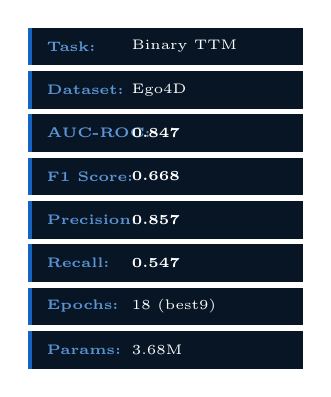
\begin{tikzpicture}
        \foreach \k/\v [count=\i] in {
          Task/Binary TTM,
          Dataset/Ego4D,
          AUC-ROC/\textbf{0.847},
          F1 Score/\textbf{0.668},
          Precision/\textbf{0.857},
          Recall/\textbf{0.547},
          Epochs/18 (best\@9),
          Params/3.68M} {
          \fill[NavyBlue!50!black] (0,{-\i*0.55}) rectangle (3.5,{-\i*0.55+0.48});
          \fill[AccBlue] (0,{-\i*0.55}) rectangle (0.06,{-\i*0.55+0.48});
          \node[right, text=AccBlue!70!white, font=\tiny\bfseries] at (0.12,{-\i*0.55+0.24}) {\k:};
          \node[right, text=white, font=\tiny] at (1.2,{-\i*0.55+0.24}) {\v};
        }
      \end{tikzpicture}
    \end{column}
  \end{columns}
\end{frame}
}

\begin{frame}{Talking To Me (TTM) Problem}
\small

\begin{columns}[T,onlytextwidth]

\begin{column}{0.46\textwidth}

\begin{tcolorbox}[
bluecard,
title={\small Formal Task Definition},
boxsep=2pt,
left=3pt,right=3pt,
top=3pt,bottom=3pt]

Given a short video clip (1--2\,sec) from an \textbf{egocentric camera}, determine whether the visible person is speaking directly to the camera wearer.

\vspace{2pt}

\begin{itemize}[leftmargin=*, itemsep=1pt]
\item[\textcolor{AccBlue}{$\blacktriangleright$}] Binary label: TTM$=1$ or TTM$=0$
\item[\textcolor{AccBlue}{$\blacktriangleright$}] Fuse visual and audio cues
\item[\textcolor{AccBlue}{$\blacktriangleright$}] Works in noisy multi-person scenes
\end{itemize}

\end{tcolorbox}

\vspace{3pt}

\begin{tcolorbox}[
orangecard,
title={\small Why not just detect speech?},
boxsep=2pt,
left=3pt,right=3pt,
top=3pt,bottom=3pt]

\begin{itemize}[leftmargin=*, itemsep=1pt]
\item Multiple people may speak simultaneously
\item Lip motion alone can fail
\item Requires audio-visual reasoning
\end{itemize}

\end{tcolorbox}

\end{column}

\begin{column}{0.52\textwidth}

\textcolor{NavyBlue}{\small\bfseries Real-World Applications}

\vspace{2pt}

\begin{tcolorbox}[
bluecard,
title={\small AR / VR Headsets},
boxsep=2pt,
left=3pt,right=3pt,
top=3pt,bottom=3pt]

\footnotesize Identify which virtual agent the user addresses.

\end{tcolorbox}

\vspace{3pt}

\begin{tcolorbox}[
tealcard,
title={\small Smart Voice Assistants},
boxsep=2pt,
left=3pt,right=3pt,
top=3pt,bottom=3pt]

\footnotesize Respond only when directly addressed.

\end{tcolorbox}

\vspace{3pt}

\begin{tcolorbox}[
orangecard,
title={\small Social Robotics \& HCI},
boxsep=2pt,
left=3pt,right=3pt,
top=3pt,bottom=3pt]

\footnotesize Enable robots to identify the correct speaker.

\end{tcolorbox}

\end{column}

\end{columns}
\end{frame}
% ── SLIDE 3: CHALLENGES ──────────────────────────────────────────────────────
\begin{frame}{Motivation \& Challenges}
\small

\begin{columns}[T,onlytextwidth]

\begin{column}{0.32\textwidth}

\begin{tcolorbox}[
redcard,
title={\small Multiple Speakers},
boxsep=2pt,
left=3pt,right=3pt,
top=3pt,bottom=3pt]

\footnotesize
3--5 people may talk simultaneously. Audio-only systems cannot determine who is addressing the wearer.

\end{tcolorbox}

\vspace{2pt}

\begin{tcolorbox}[
tealcard,
title={\small Audio-Visual Sync Issues},
boxsep=2pt,
left=3pt,right=3pt,
top=3pt,bottom=3pt]

\footnotesize
Egocentric recordings may contain small A-V timing offsets due to hardware buffering.

\end{tcolorbox}

\end{column}

\begin{column}{0.32\textwidth}

\begin{tcolorbox}[
bluecard,
title={\small Occlusions \& Camera Motion},
boxsep=2pt,
left=3pt,right=3pt,
top=3pt,bottom=3pt]

\footnotesize
First-person cameras move with the wearer. Faces may blur, disappear, or leave the frame.

\end{tcolorbox}

\vspace{2pt}

\begin{tcolorbox}[
orangecard,
title={\small Class Imbalance},
boxsep=2pt,
left=3pt,right=3pt,
top=3pt,bottom=3pt]

\footnotesize
Only a small fraction of clips correspond to TTM$=1$, making training biased toward negative samples.

\end{tcolorbox}

\end{column}

\begin{column}{0.32\textwidth}

\begin{tcolorbox}[
purplecard,
title={\small Lip Movement Ambiguity},
boxsep=2pt,
left=3pt,right=3pt,
top=3pt,bottom=3pt]

\footnotesize
Lip motion does not always indicate speech. People may whisper, laugh, or mouth words silently.

\end{tcolorbox}

\vspace{2pt}

\begin{tcolorbox}[
purplecard,
title={\small Pre-training Domain Gap},
boxsep=2pt,
left=3pt,right=3pt,
top=3pt,bottom=3pt]

\footnotesize
Pretrained backbones differ significantly from real-world egocentric social interactions.

\end{tcolorbox}

\end{column}

\end{columns}

\vspace{3pt}

\begin{tcolorbox}[
bluecard,
boxsep=2pt,
left=3pt,right=3pt,
top=3pt,bottom=3pt]

\small
\textbf{Conclusion:} Audio-only or video-only systems are insufficient. 
Robust TTM detection requires multimodal fusion with temporal modeling.

\end{tcolorbox}

\end{frame}

% ── SLIDE 4: DATASET ─────────────────────────────────────────────────────────
\begin{frame}{Dataset Overview}
\small

\begin{columns}[T,onlytextwidth]

\begin{column}{0.46\textwidth}

\begin{tcolorbox}[
bluecard,
title={\small About Ego4D TTM},
boxsep=2pt,
left=3pt,right=3pt,
top=3pt,bottom=3pt]

\footnotesize
\begin{itemize}[leftmargin=*, itemsep=1pt]
  \item Large-scale egocentric real-world video dataset
  \item Binary TTM label for each visible face
  \item Video: 30 FPS, 1080p \quad Audio: 16\,kHz
  \item Professionally annotated labels
  \item Used balanced 70k subset for training
\end{itemize}

\end{tcolorbox}

\vspace{3pt}

\centering
\begin{tikzpicture}[scale=0.78]

\foreach \num/\lbl/\col [count=\i] in {
700+/Hours Ego Video/AccBlue,
70k/Training Clips/AccTeal,
6390/Test Clips/AccOrange
} {

\fill[LightBg] ({(\i-1)*2.35},0) rectangle ({(\i-1)*2.35+2.15},0.9);
\fill[\col] ({(\i-1)*2.35},0) rectangle ({(\i-1)*2.35+2.15},0.06);

\node[font=\bfseries\small,text=\col]
at ({(\i-1)*2.35+1.07},0.58) {\num};

\node[font=\tiny,text=MidText,align=center]
at ({(\i-1)*2.35+1.07},0.22) {\lbl};
}

\end{tikzpicture}

\end{column}

\begin{column}{0.52\textwidth}

\textcolor{NavyBlue}{\small\bfseries Evaluation Metrics}

\vspace{2pt}

\begin{tcolorbox}[
bluecard,
title={\small AUC-ROC},
boxsep=2pt,
left=3pt,right=3pt,
top=3pt,bottom=3pt]

\footnotesize
Measures model discrimination across all thresholds.
AUC$=0.5$ is random while AUC$=1.0$ is perfect.

\textbf{Result: 0.847}

\end{tcolorbox}

\vspace{2pt}

\begin{tcolorbox}[
tealcard,
title={\small Binary F1 Score},
boxsep=2pt,
left=3pt,right=3pt,
top=3pt,bottom=3pt]

\footnotesize
Balances Precision and Recall for the TTM$=1$ class.
Important due to class imbalance.

\textbf{Result: F1 = 0.668}

\end{tcolorbox}

\vspace{2pt}

\begin{tcolorbox}[
orangecard,
title={\small Precision \& Recall},
boxsep=2pt,
left=3pt,right=3pt,
top=3pt,bottom=3pt]

\footnotesize
Precision reduces false alarms, while Recall measures how many true TTM events are detected.

\textbf{Precision: 0.857 \quad Recall: 0.547}

\end{tcolorbox}

\end{column}

\end{columns}
\end{frame}
% ── SLIDE 5: ARCHITECTURE ────────────────────────────────────────────────────

\begin{frame}{Complete Pipeline Architecture}
\centering
\resizebox{\textwidth}{!}{%

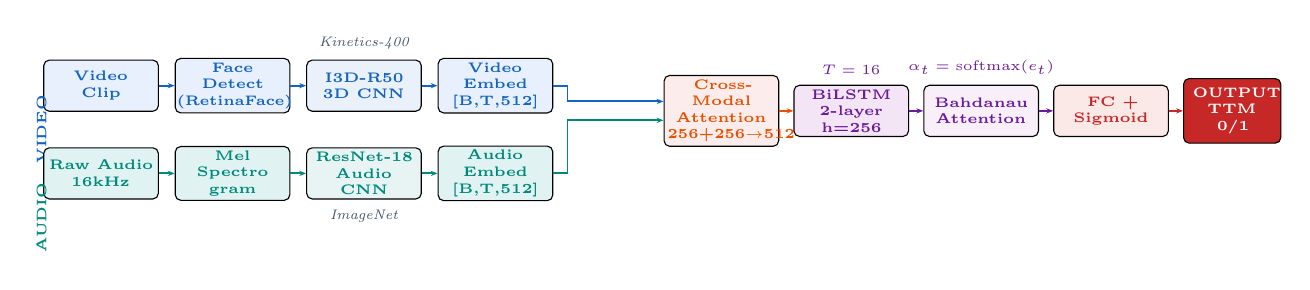
\begin{tikzpicture}[
    node distance=0.18cm and 0.2cm,
    box/.style={
        draw,
        rounded corners=2pt,
        fill=#1,
        text width=1.35cm,
        minimum height=0.65cm,
        align=center,
        font=\tiny\bfseries,
        inner sep=1.5pt
    },
    arr/.style={-{Stealth[length=2.5pt]}, line width=0.7pt, color=#1},
    every node/.style={font=\tiny}
]

% VIDEO ROW
\node[box=CardBlue, text=AccBlue] (vc) {Video\\Clip};

\node[box=CardBlue, text=AccBlue, right=of vc] (fd)
{Face Detect\\(RetinaFace)};

\node[box=CardBlue!60!AccBlue!20!, text=AccBlue, right=of fd] (cnn3d)
{\textbf{I3D-R50}\\3D CNN};

\node[box=CardBlue, text=AccBlue, right=of cnn3d] (ve)
{Video Embed\\{[B,T,512]}};

\draw[arr=AccBlue] (vc) -- (fd);
\draw[arr=AccBlue] (fd) -- (cnn3d);
\draw[arr=AccBlue] (cnn3d) -- (ve);

\node[rotate=90, text=AccBlue, font=\tiny\bfseries,
left=0.02cm of vc] {VIDEO};

% AUDIO ROW
\node[box=CardTeal, text=AccTeal, below=0.45cm of vc] (ra)
{Raw Audio\\16kHz};

\node[box=CardTeal, text=AccTeal, right=of ra] (ms)
{Mel Spectro\\gram};

\node[box=CardTeal!60!AccTeal!20!, text=AccTeal, right=of ms] (acnn)
{\textbf{ResNet-18}\\Audio CNN};

\node[box=CardTeal, text=AccTeal, right=of acnn] (ae)
{Audio Embed\\{[B,T,512]}};

\draw[arr=AccTeal] (ra) -- (ms);
\draw[arr=AccTeal] (ms) -- (acnn);
\draw[arr=AccTeal] (acnn) -- (ae);

\node[rotate=90, text=AccTeal, font=\tiny\bfseries,
left=0.02cm of ra] {AUDIO};

% FUSION
\node[box=CardOrange!80!, text=AccOrange,
right=1.4cm of ve, yshift=-0.32cm] (xattn)
{\textbf{Cross-Modal}\\Attention\\256+256$\to$512};

\node[box=CardPurple, text=AccPurple,
right=0.18cm of xattn] (bilstm)
{\textbf{BiLSTM}\\2-layer\\h=256};

\node[box=CardPurple!60!, text=AccPurple,
right=0.18cm of bilstm] (attn)
{\textbf{Bahdanau}\\Attention};

\node[box=CardOrange, text=AccRed,
right=0.18cm of attn] (fc)
{\textbf{FC +}\\Sigmoid};

\node[
draw,
fill=AccRed,
text=white,
rounded corners=2pt,
right=0.18cm of fc,
minimum height=0.45cm,
font=\tiny\bfseries,
text width=1cm,
align=center
] (out)
{OUTPUT\\TTM 0/1};

\draw[arr=AccOrange] (xattn) -- (bilstm);
\draw[arr=AccPurple] (bilstm) -- (attn);
\draw[arr=AccPurple] (attn) -- (fc);
\draw[arr=AccRed] (fc) -- (out);

% CONNECTIONS
\draw[arr=AccBlue]
(ve.east) -- ++(0.18,0)
|- ([yshift=0.12cm]xattn.west);

\draw[arr=AccTeal]
(ae.east) -- ++(0.18,0)
|- ([yshift=-0.12cm]xattn.west);

% LABELS
\node[above=0.01cm of cnn3d,
font=\tiny\itshape,
text=MidText]
{Kinetics-400};

\node[below=0.01cm of acnn,
font=\tiny\itshape,
text=MidText]
{ImageNet};

\node[above=0.01cm of bilstm,
font=\tiny,
text=AccPurple]
{$T=16$};

\node[above=0.01cm of attn,
font=\tiny,
text=AccPurple]
{$\alpha_t=\text{softmax}(e_t)$};

\end{tikzpicture}
}

\vspace{2pt}

\begin{tcolorbox}[
bluecard,
boxsep=2pt,
left=3pt,right=3pt,
top=3pt,bottom=3pt]

\scriptsize
\textbf{Balanced Test Results:}
AUC-ROC = \textbf{0.847} \quad
F1 = \textbf{0.668} \quad
Precision = \textbf{0.857}

Recall = \textbf{0.547} \quad
Accuracy = \textbf{72.8\%} \quad
Parameters = \textbf{3.68M}

\end{tcolorbox}

\end{frame}
% ── SLIDE 6: VIDEO PIPELINE ──────────────────────────────────────────────────
\begin{frame}{Video Processing Pipeline}

\textcolor{NavyBlue}{\footnotesize
I3D-R50 used in fusion model \hfill SlowFast-R50 evaluated as standalone baseline}

\vspace{3pt}

\small

\begin{columns}[T,onlytextwidth]

\begin{column}{0.48\textwidth}

\begin{tcolorbox}[
bluecard,
title={\small Why 3D CNN? Why SlowFast?},
boxsep=2pt,
left=3pt,right=3pt,
top=3pt,bottom=3pt]

\footnotesize
\begin{itemize}[leftmargin=*, itemsep=1pt]
  \item 2D CNNs process frames independently
  \item 3D convolutions learn spatial + temporal motion
  \item \textbf{SlowFast dual-pathway:}
  \begin{itemize}[leftmargin=*]
    \item \textcolor{AccBlue}{SLOW (4 FPS):} appearance features
    \item \textcolor{AccTeal}{FAST (32 FPS):} motion features
  \end{itemize}
  \item Slow + Fast fused using lateral connections
  \item Pretrained on Kinetics-400
  \item Output: \textbf{512-dim video embedding}
\end{itemize}

\end{tcolorbox}

\end{column}

\begin{column}{0.50\textwidth}

\begin{tcolorbox}[
bluecard,
title={\small SLOW Pathway},
boxsep=2pt,
left=3pt,right=3pt,
top=3pt,bottom=3pt]

\footnotesize
\begin{itemize}[leftmargin=*, itemsep=1pt]
  \item 4 FPS, 8 frames/clip
  \item High spatial resolution
  \item Learns semantic facial features
\end{itemize}

\end{tcolorbox}

\vspace{2pt}

\begin{tcolorbox}[
tealcard,
title={\small FAST Pathway},
boxsep=2pt,
left=3pt,right=3pt,
top=3pt,bottom=3pt]

\footnotesize
\begin{itemize}[leftmargin=*, itemsep=1pt]
  \item 32 FPS temporal stream
  \item Lightweight architecture
  \item Captures rapid lip and jaw motion
\end{itemize}

\end{tcolorbox}

\vspace{2pt}

\begin{tcolorbox}[
orangecard,
title={\small Training Observation},
boxsep=2pt,
left=3pt,right=3pt,
top=3pt,bottom=3pt]

\footnotesize
Video-only SlowFast model showed severe overfitting.
Fine-tuning only the final blocks improved generalization.

\end{tcolorbox}

\end{column}

\end{columns}

\end{frame}
% ── SLIDE 7: AUDIO PIPELINE ──────────────────────────────────────────────────
\begin{frame}{Audio Processing Pipeline}
\small

\textcolor{NavyBlue}{\footnotesize\bfseries
Mel Spectrogram + ResNet-18 CNN \hfill Best audio-only val\_acc: 66.78\%}

\vspace{3pt}

\begin{columns}[T,onlytextwidth]

\begin{column}{0.49\textwidth}

\begin{tcolorbox}[
tealcard,
title={\small Step 1 --- Audio Extraction},
boxsep=2pt,
left=3pt,right=3pt,
top=3pt,bottom=3pt]

\footnotesize
Extract 16\,kHz mono audio and segment into 1-sec windows aligned with video clips.

\end{tcolorbox}

\vspace{2pt}

\begin{tcolorbox}[
tealcard,
title={\small Step 2 --- Mel Spectrogram},
boxsep=2pt,
left=3pt,right=3pt,
top=3pt,bottom=3pt]

\footnotesize
Apply STFT and convert to 64 Mel bands.
Final spectrogram size: \textbf{[1,64,50]}.

\end{tcolorbox}

\vspace{2pt}

\begin{tcolorbox}[
orangecard,
title={\small Why Mel Scale?},
boxsep=2pt,
left=3pt,right=3pt,
top=3pt,bottom=3pt]

\footnotesize
Mel scale models human auditory perception and helps CNNs learn speech-relevant frequency patterns efficiently.

\end{tcolorbox}

\end{column}

\begin{column}{0.49\textwidth}

\begin{tcolorbox}[
tealcard,
title={\small Step 3 --- ResNet-18 Audio CNN},
boxsep=2pt,
left=3pt,right=3pt,
top=3pt,bottom=3pt]

\footnotesize
Treat spectrogram as a 1-channel image.
ImageNet-pretrained ResNet-18 extracts spectral and speech-related features.

\textbf{Best audio-only val\_acc: 66.78\%}

\end{tcolorbox}

\vspace{2pt}

\begin{tcolorbox}[
tealcard,
title={\small Step 4 --- Audio Embedding},
boxsep=2pt,
left=3pt,right=3pt,
top=3pt,bottom=3pt]

\footnotesize
Global Average Pooling produces a \textbf{512-dim embedding} aligned with video features.

\end{tcolorbox}

\vspace{2pt}

\begin{tcolorbox}[
purplecard,
title={\small Training Observation},
boxsep=2pt,
left=3pt,right=3pt,
top=3pt,bottom=3pt]

\footnotesize
Audio CNN overfit quickly.
BiLSTM-based temporal modeling improved utilization of audio features.

\end{tcolorbox}

\end{column}

\end{columns}
\end{frame}

% ── SLIDE 8: BILSTM ──────────────────────────────────────────────────────────
\begin{frame}{Temporal Modeling with BiLSTM}

\textcolor{NavyBlue}{\footnotesize
Bidirectional LSTM --- Hidden size: 256 per direction $\rightarrow$ 512 total}

\vspace{3pt}

\small

\begin{columns}[T,onlytextwidth]

\begin{column}{0.47\textwidth}

\begin{tcolorbox}[
bluecard,
title={\small Why Temporal Modeling?},
boxsep=2pt,
left=3pt,right=3pt,
top=3pt,bottom=3pt]

\footnotesize
\begin{itemize}[leftmargin=*, itemsep=1pt]
  \item Cross-modal attention gives one fused feature per clip
  \item Speech evolves continuously over time
  \item Stack $T=16$ consecutive clips into a sequence
  \item Forward pass uses past context
  \item Backward pass uses future context
  \item Outputs 512-dim temporal representation
  \item 2 stacked BiLSTM layers improve abstraction
\end{itemize}

\end{tcolorbox}

\end{column}

\begin{column}{0.51\textwidth}

\textcolor{NavyBlue}{\small\bfseries Actual Configuration}

\vspace{2pt}

\scriptsize

\begin{tabular}{@{}p{2.8cm}p{3.8cm}@{}}
\toprule

\rowcolor{NavyBlue}
\color{white}\bfseries Parameter &
\color{white}\bfseries Value \\

\midrule

\rowcolor{CardBlue}
Input dim & 512 fused features \\

Hidden size & 256 per direction \\

\rowcolor{CardBlue}
Layers & 2 stacked BiLSTM \\

Sequence length & $T=16$ clips \\

\rowcolor{CardBlue}
Train stride & 4 clips \\

Inference stride & 8 clips \\

\rowcolor{CardBlue}
Dropout & 0.5 \\

Total params & 3.68M \\

\bottomrule
\end{tabular}

\vspace{3pt}

\begin{tcolorbox}[
tealcard,
boxsep=2pt,
left=3pt,right=3pt,
top=3pt,bottom=3pt]

\footnotesize
\textbf{Intuition:}
BiLSTM accumulates evidence across consecutive clips, improving robustness compared to isolated clip predictions.

\end{tcolorbox}

\end{column}

\end{columns}

\end{frame}
%================================================
\begin{frame}{Bahdanau Attention Mechanism}

\textcolor{NavyBlue}{\footnotesize
Learning to focus on the most informative time steps}

\vspace{3pt}

\small

\begin{columns}[T,onlytextwidth]

\begin{column}{0.43\textwidth}

\begin{tcolorbox}[
purplecard,
title={\small What Does Attention Solve?},
boxsep=2pt,
left=3pt,right=3pt,
top=3pt,bottom=3pt]

\footnotesize
\begin{itemize}[leftmargin=*, itemsep=1pt]
  \item BiLSTM outputs $T=16$ hidden states
  \item Mean pooling treats all clips equally
  \item Attention assigns weight $\alpha_t$ to each step
  \item $\sum_t \alpha_t = 1$
  \item Weighted context vector goes to classifier
  \item Fully trainable end-to-end
\end{itemize}

\end{tcolorbox}

\vspace{0.5pt}

\begin{tcolorbox}[
purplecard,
title={\small Bahdanau Equations},
boxsep=1pt,
left=3pt,right=3pt,
top=1pt,bottom=1pt]

\scriptsize
\begin{align*}
e_t &= v^\top \tanh(W h_t + b) \\
\alpha_t &= \frac{\exp(e_t)}{\sum_j \exp(e_j)} \\
c &= \sum_{t=1}^{T} \alpha_t h_t
\end{align*}

\end{tcolorbox}

\end{column}

\begin{column}{0.55\textwidth}

\textcolor{NavyBlue}{\small\bfseries Attention Weight Distribution}

\vspace{2pt}

{\tiny High attention weights indicate important clips for prediction.}

\vspace{2pt}

\centering

\resizebox{0.95\linewidth}{!}{
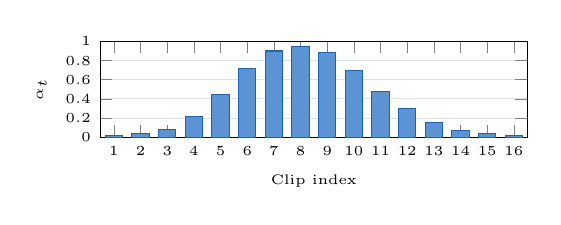
\begin{tikzpicture}

\pgfplotsset{
every axis/.append style={
width=7cm,
height=2.8cm,
ymin=0,
ymax=1,
xmin=0.5,
xmax=16.5,
xtick={1,2,...,16},
xticklabel style={font=\tiny},
yticklabel style={font=\tiny},
xlabel style={font=\tiny},
ylabel style={font=\tiny},
xlabel={Clip index},
ylabel={$\alpha_t$},
ymajorgrids=true,
grid style={LightLine!70},
}
}

\begin{axis}

\addplot[
ybar,
bar width=0.22cm,
fill=AccBlue!70,
draw=AccBlue]
coordinates {
(1,0.02)(2,0.04)(3,0.08)(4,0.22)
(5,0.45)(6,0.72)(7,0.90)(8,0.95)
(9,0.88)(10,0.70)(11,0.48)(12,0.30)
(13,0.15)(14,0.07)(15,0.04)(16,0.02)
};

\end{axis}
\end{tikzpicture}
}

\vspace{2pt}

{\footnotesize\color{AccPurple}
High attention during clips with synchronized lip motion and audio activity.}

\vspace{2pt}

\begin{tcolorbox}[
purplecard,
boxsep=2pt,
left=3pt,right=3pt,
top=3pt,bottom=3pt]

\footnotesize
\textbf{Key benefit:}
Attention improves interpretability by identifying which clips influenced the prediction most.

\end{tcolorbox}

\end{column}

\end{columns}

\end{frame}

% ── SLIDE 10: TRAINING STRATEGY ──────────────────────────────────────────────
\begin{frame}{Training Strategy}

\textcolor{NavyBlue}{\footnotesize
Actual configuration from \texttt{metrics.json}}

\vspace{2pt}

\small

\begin{columns}[T,onlytextwidth]

% LEFT COLUMN
\begin{column}{0.45\textwidth}

\textcolor{NavyBlue}{\small\bfseries Training Configuration}

\vspace{2pt}

\scriptsize

\begin{tabular}{@{}p{2.3cm}p{3.5cm}@{}}

\toprule

\rowcolor{NavyBlue}
\color{white}\bfseries Parameter &
\color{white}\bfseries Value \\

\midrule

\rowcolor{CardBlue}
Fusion type & Cross-attention \\

Loss & Weighted BCE \\

\rowcolor{CardBlue}
Optimizer & AdamW ($3\times10^{-4}$) \\

LR Scheduler & ReduceLROnPlateau \\

\rowcolor{CardBlue}
Batch size & 256 \\

Sampler & Weighted sampler \\

\rowcolor{CardBlue}
Dropout & 0.5 \\

Sequence length & $T=16$ \\

\rowcolor{CardBlue}
Best epoch & 9 \\

Total epochs & 18 \\

\rowcolor{CardBlue}
Threshold & 0.139 \\

\bottomrule

\end{tabular}

\end{column}

% RIGHT COLUMN
\begin{column}{0.53\textwidth}

\textcolor{NavyBlue}{\small\bfseries Training Curves}

\vspace{1pt}

\centering

\resizebox{0.98\linewidth}{!}{
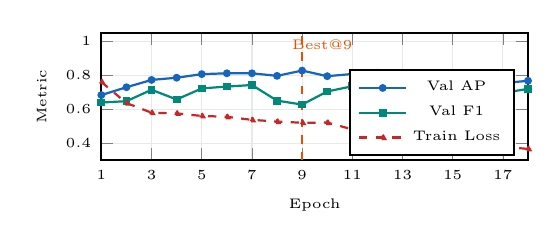
\begin{tikzpicture}

\begin{axis}[
width=7cm,
height=3.2cm,
xlabel=Epoch,
ylabel=Metric,
xmin=1,
xmax=18,
ymin=0.3,
ymax=1.05,
xtick={1,3,5,7,9,11,13,15,17},
legend pos=south east,
legend style={font=\tiny},
grid=major,
grid style={LightLine!50},
tick label style={font=\tiny},
label style={font=\tiny},
line width=0.8pt,
]

\addplot[
color=AccBlue,
mark=*,
mark size=1pt]
coordinates {
(1,0.684)(2,0.730)(3,0.773)(4,0.786)
(5,0.807)(6,0.812)(7,0.812)(8,0.797)
(9,0.828)(10,0.795)(11,0.808)(12,0.815)
(13,0.793)(14,0.777)(15,0.776)(16,0.788)
(17,0.754)(18,0.768)};

\addlegendentry{Val AP}

\addplot[
color=AccTeal,
mark=square*,
mark size=1pt]
coordinates {
(1,0.640)(2,0.648)(3,0.715)(4,0.658)
(5,0.723)(6,0.734)(7,0.743)(8,0.651)
(9,0.628)(10,0.705)(11,0.736)(12,0.686)
(13,0.752)(14,0.708)(15,0.715)(16,0.679)
(17,0.697)(18,0.720)};

\addlegendentry{Val F1}

\addplot[
color=AccRed,
dashed,
mark=triangle*,
mark size=1pt]
coordinates {
(1,0.761)(2,0.637)(3,0.580)(4,0.576)
(5,0.561)(6,0.556)(7,0.538)(8,0.528)
(9,0.521)(10,0.522)(11,0.482)(12,0.457)
(13,0.455)(14,0.405)(15,0.431)(16,0.394)
(17,0.380)(18,0.367)};

\addlegendentry{Train Loss}

\draw[AccOrange,dashed,line width=0.7pt]
(axis cs:9,0.3) -- (axis cs:9,1.05);

\node[font=\tiny,text=AccOrange]
at (axis cs:9.8,0.98) {Best@9};

\end{axis}
\end{tikzpicture}
}

\vspace{1pt}

\begin{tcolorbox}[
orangecard,
boxsep=1pt,
left=2pt,right=2pt,
top=2pt,bottom=2pt]

\footnotesize
Validation AP plateaued after epoch 9 while train loss kept decreasing, indicating overfitting and motivating early stopping.

\end{tcolorbox}

\end{column}

\end{columns}

\end{frame}
% ── SLIDE 11: EXPERIMENTAL RESULTS ───────────────────────────────────────────
\begin{frame}{Experimental Results}

\textcolor{NavyBlue}{\footnotesize
Evaluation results from fusion model experiments}

\vspace{2pt}

\small

\begin{columns}[T,onlytextwidth]

% LEFT COLUMN
\begin{column}{0.50\textwidth}

\textcolor{NavyBlue}{\small\bfseries Balanced Test Set}

\vspace{2pt}

\begin{columns}[T]

\begin{column}{0.24\textwidth}
\metricbox{0.847}{AUC-ROC}{Balanced test}{AccBlue}
\end{column}

\begin{column}{0.24\textwidth}
\metricbox{0.668}{F1 Score}{TTM class}{AccTeal}
\end{column}

\begin{column}{0.24\textwidth}
\metricbox{0.857}{Precision}{Low FP}{AccOrange}
\end{column}

\begin{column}{0.24\textwidth}
\metricbox{0.547}{Recall}{Needs improvement}{AccRed}
\end{column}

\end{columns}

\vspace{3pt}

\textcolor{NavyBlue}{\small\bfseries Confusion Matrix}

\vspace{2pt}

\scriptsize

\begin{tabular}{@{}lcc@{}}

\toprule

\rowcolor{NavyBlue}
& \color{white}\small Pred: Non-TTM
& \color{white}\small Pred: TTM \\

\midrule

\rowcolor{CardGreen}
\small\bfseries Actual: Non-TTM &
\cellcolor{CardGreen}\textbf{TN = 5807} &
\cellcolor{CardOrange}FP = 583 \\

\rowcolor{CardOrange}
\small\bfseries Actual: TTM &
\cellcolor{CardOrange}FN = 2893 &
\cellcolor{CardGreen}\textbf{TP = 3497} \\

\bottomrule

\end{tabular}

\vspace{2pt}

{\scriptsize\color{MidText}
High precision but relatively lower recall.}

\end{column}

% RIGHT COLUMN
\begin{column}{0.39\textwidth}

\textcolor{NavyBlue}{\small\bfseries Component Comparison}

\vspace{2pt}

\scriptsize

\begin{tabular}{@{}lcc@{}}

\toprule

\rowcolor{NavyBlue}
\color{white}\small Model &
\color{white}\small Acc &
\color{white}\small AUC \\

\midrule

\rowcolor{CardOrange}
SlowFast only & 61.9\% & --- \\

Audio CNN only & 66.8\% & --- \\

\rowcolor{CardGreen}
\bfseries Full Fusion &
\bfseries 72.8\% &
\bfseries 0.847 \\

\bottomrule

\end{tabular}

\vspace{4pt}

\textcolor{NavyBlue}{\small\bfseries Validation Set}

\vspace{2pt}

\scriptsize

\begin{tabular}{@{}lc@{}}

\toprule

\rowcolor{NavyBlue}
\color{white}\small Metric &
\color{white}\small Value \\

\midrule

\rowcolor{CardBlue}
AUC-ROC & 0.995 \\

F1 Score & 0.797 \\

\rowcolor{CardBlue}
Precision & 0.693 \\

Recall & 0.937 \\

\rowcolor{CardBlue}
Accuracy & 98.2\% \\

\bottomrule

\end{tabular}

\vspace{3pt}

\begin{tcolorbox}[
orangecard,
boxsep=1pt,
left=2pt,right=2pt,
top=2pt,bottom=2pt]

\footnotesize
Validation performance appears inflated because the validation split is highly imbalanced.

\end{tcolorbox}

\end{column}

\end{columns}

\end{frame}
%======================================
% =====================================================================
% Slide: Comparison with Prior Work
% Drop this between your "Experimental Results" and "Risks & Mitigation"
% slides. Requires: booktabs, array, xcolor, tcolorbox (or adjust boxes).
% =====================================================================

% =====================================================================
% Slide: Comparison with Prior Work (v2 — with accuracy + explanation)
% Place between "Experimental Results" and "Risks & Mitigation".
% Requires: booktabs, array, xcolor. tcolorbox optional.
% =====================================================================

% =====================================================================
% Slide: Comparison with Prior Work (v3)
% Table format: Paper | Method Used | Accuracy | Parameters
% Place between "Experimental Results" and "Risks & Mitigation".
% Requires: booktabs, array, xcolor.
% =====================================================================

\begin{frame}{Comparison with Prior Work}

% -------------------- COMPARISON TABLE --------------------
\begin{center}
\scriptsize
\renewcommand{\arraystretch}{1.3}
\setlength{\tabcolsep}{6pt}
\begin{tabular}{@{}p{2.5cm} p{4.6cm} p{2.0cm} p{1.2cm}@{}}
\toprule
\textbf{Paper} & \textbf{Method Used} & \textbf{Accuracy} & \textbf{Params}\\
\midrule
TalkNet \newline\textit{(Tao et al., '21)}
 & 3D-ResNet visual + audio CNN $+$ self-attention temporal encoder (AVA-ASD)
 & 92.3 (mAP) & 15.0M \\

ASDNet \newline\textit{(Köpüklü et al., '21)}
 & 3D-ResNeXt-101 visual + SincDSNet audio $+$ stacked GRU (AVA-ASD)
 & 93.5 (mAP) & 49.7M \\

MAAS \newline\textit{(Alcázar et al., '21)}
 & 2D-ResNet-18 features $+$ multi-modal graph (GCN) reasoning (AVA-ASD)
 & 88.8 (mAP) & 21.7M \\

Light-ASD \newline\textit{(Liao et al., '23)}
 & Lightweight 3D visual + audio encoders $+$ BiGRU (AVA-ASD)
 & 94.1 (mAP) & 1.0M  \\

Ego4D Baseline \newline\textit{(Grauman et al., '22)}
 & 2D ResNet-18 face crops $+$ audio CNN $+$ mean pooling (Ego4D TTM)
 & $\sim$60\% (Acc) & $\sim$11M \\

\rowcolor{green!15}
\textbf{Ours} \newline\textbf{(Group 42, '25)}
 & \textbf{I3D-R50 visual + ResNet-18 audio $+$ cross-modal attention $+$ BiLSTM + Bahdanau attention (Ego4D TTM)}
 & \textbf{72.8\% (Acc)} \newline \textbf{0.847 (AUC)} & \textbf{3.68M} \\
\bottomrule
\end{tabular}
\end{center}



\vspace{0.2em}
\scriptsize
\textbf{Key takeaways:}
\textbf{(1)} Ours is the only \emph{egocentric} model that uses both
\emph{cross-modal attention} and a \emph{two-stage} (cross-attn + Bahdanau)
attention design.
\textbf{(2)} We achieve competitive accuracy with \textbf{3.68M params} ---
4--13$\times$ smaller than TalkNet / ASDNet / MAAS.
\textbf{(3)} Imbalance-aware training (weighted BCE + sampler + threshold
$0.139$) directly targets the TTM class skew that prior ASD methods do not address.

\end{frame}

% ── SLIDE 12: RISKS & MITIGATIONS ────────────────────────────────────────────
\begin{frame}{Risks \& Mitigation Strategies}

\textcolor{NavyBlue}{\footnotesize
Known challenges encountered during development}

\vspace{2pt}

\small

\begin{columns}[T,onlytextwidth]

% COLUMN 1
\begin{column}{0.32\textwidth}

\begin{tcolorbox}[
redcard,
title={\small GPU Memory (OOM)},
boxsep=1pt,
left=2pt,right=2pt,
top=2pt,bottom=2pt]

\footnotesize
\textbf{Problem:}
3D CNN + BiLSTM exceeded GPU memory.

\textbf{Fix:}
FP16 mixed precision, gradient accumulation, reduced resolution.

\end{tcolorbox}

\vspace{2pt}

\begin{tcolorbox}[
redcard,
title={\small Low Recall},
boxsep=1pt,
left=2pt,right=2pt,
top=2pt,bottom=2pt]

\footnotesize
\textbf{Problem:}
Model missed many true TTM events.

\textbf{Fix:}
Threshold tuning and future transformer-based modeling.

\end{tcolorbox}

\end{column}

% COLUMN 2
\begin{column}{0.32\textwidth}

\begin{tcolorbox}[
purplecard,
title={\small Video CNN Overfitting},
boxsep=1pt,
left=2pt,right=2pt,
top=2pt,bottom=2pt]

\footnotesize
\textbf{Observed:}
Training accuracy saturated quickly.

\textbf{Fix:}
Dropout, weight decay, freezing early layers, early stopping.

\end{tcolorbox}

\vspace{2pt}

\begin{tcolorbox}[
purplecard,
title={\small Gradient Vanishing},
boxsep=1pt,
left=2pt,right=2pt,
top=2pt,bottom=2pt]

\footnotesize
\textbf{Problem:}
BiLSTM gradients weakened over long sequences.

\textbf{Fix:}
Gradient clipping and attention-based shortcuts.

\end{tcolorbox}

\end{column}

% COLUMN 3
\begin{column}{0.32\textwidth}

\begin{tcolorbox}[
orangecard,
title={\small Class Imbalance},
boxsep=1pt,
left=2pt,right=2pt,
top=2pt,bottom=2pt]

\footnotesize
\textbf{Problem:}
TTM-positive samples were limited.

\textbf{Fix:}
Weighted sampling and monitoring F1/AUC instead of accuracy.

\end{tcolorbox}

\vspace{2pt}

\begin{tcolorbox}[
tealcard,
title={\small Audio-Visual Sync},
boxsep=1pt,
left=2pt,right=2pt,
top=2pt,bottom=2pt]

\footnotesize
\textbf{Problem:}
Small audio-video timing offsets existed.

\textbf{Fix:}
Synchronization checks and temporal augmentation.

\end{tcolorbox}

\end{column}

\end{columns}

\end{frame}


%=====================================
\begin{frame}{Team Role Distribution}

\textcolor{NavyBlue}{\footnotesize
Group 42 --- Component-wise contribution distribution}

\vspace{2pt}

\small

\begin{columns}[T,onlytextwidth]

% LEFT COLUMN
\begin{column}{0.52\textwidth}

\scriptsize

\resizebox{\linewidth}{!}{
\begin{tabular}{@{}p{2.0cm}p{1.8cm}p{2.8cm}@{}}

\toprule

\rowcolor{NavyBlue}
\color{white}\small\bfseries Members &
\color{white}\small\bfseries Role &
\color{white}\small\bfseries Contribution \\

\midrule

\rowcolor{CardBlue}
Mihir + Harshit &
3D Video CNN &
I3D / SlowFast-R50 pipeline \\

Aman + Kanika &
Video Prep &
Frame extraction and preprocessing \\

\rowcolor{CardTeal}
Naman + Sowmika &
Audio CNN &
Mel spectrogram + ResNet-18 \\

Vikky + Vershita &
BiLSTM + Attention &
Temporal modeling and attention \\

\rowcolor{CardOrange}
Vershita + Vikky &
Training &
Training loop and optimization \\

\bottomrule

\end{tabular}
}

\end{column}

% RIGHT COLUMN
\begin{column}{0.39\textwidth}

\textcolor{NavyBlue}{\small\bfseries Component Ownership Diagram}

\vspace{2pt}

\centering

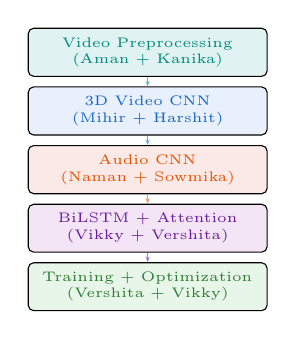
\begin{tikzpicture}

\tikzset{
comp/.style args={#1}{
draw,
rounded corners=2pt,
fill=#1,
text width=2.8cm,
minimum height=0.58cm,
align=center,
font=\tiny
}
}

\node[comp=CardTeal, text=AccTeal] (prep)
{Video Preprocessing\\(Aman + Kanika)};

\node[comp=CardBlue, text=AccBlue,
below=0.12cm of prep] (v)
{3D Video CNN\\(Mihir + Harshit)};

\node[comp=CardOrange, text=AccOrange,
below=0.12cm of v] (a)
{Audio CNN\\(Naman + Sowmika)};

\node[comp=CardPurple, text=AccPurple,
below=0.12cm of a] (b)
{BiLSTM + Attention\\(Vikky + Vershita)};

\node[comp=CardGreen, text=AccGreen,
below=0.12cm of b] (t)
{Training + Optimization\\(Vershita + Vikky)};

\draw[-{Stealth[length=2pt]}, AccTeal!60] (prep) -- (v);
\draw[-{Stealth[length=2pt]}, AccBlue!60] (v) -- (a);
\draw[-{Stealth[length=2pt]}, AccOrange!60] (a) -- (b);
\draw[-{Stealth[length=2pt]}, AccPurple!60] (b) -- (t);

\end{tikzpicture}

\end{column}

\end{columns}

\end{frame}

% ── SLIDE 15: CONCLUSION ─────────────────────────────────────────────────────

\begin{frame}{Conclusion \& Future Work}

\textcolor{NavyBlue}{\footnotesize
Key findings from the Ego4D TTM benchmark and future directions}

\vspace{2pt}

\small

\begin{columns}[T,onlytextwidth]

% LEFT COLUMN
\begin{column}{0.49\textwidth}

\textcolor{NavyBlue}{\small\bfseries Key Conclusions}

\vspace{2pt}

\begin{tcolorbox}[
bluecard,
title={\small Multimodal Fusion},
boxsep=1pt,
left=2pt,right=2pt,
top=2pt,bottom=2pt]

\footnotesize
Video-only and audio-only models underperformed compared to the full fusion model, proving both modalities are essential.

\end{tcolorbox}

\vspace{2pt}

\begin{tcolorbox}[
tealcard,
title={\small Cross-Modal Attention},
boxsep=1pt,
left=2pt,right=2pt,
top=2pt,bottom=2pt]

\footnotesize
Cross-modal attention improved interaction between audio and video features before temporal modeling.

\end{tcolorbox}

\vspace{2pt}

\begin{tcolorbox}[
purplecard,
title={\small Temporal Context},
boxsep=1pt,
left=2pt,right=2pt,
top=2pt,bottom=2pt]

\footnotesize
BiLSTM effectively modeled sustained speech behavior across multiple clips.

\end{tcolorbox}

\vspace{2pt}

\begin{tcolorbox}[
orangecard,
title={\small Precision vs Recall},
boxsep=1pt,
left=2pt,right=2pt,
top=2pt,bottom=2pt]

\footnotesize
The model achieved high precision with moderate recall, highlighting the need for threshold optimization.

\end{tcolorbox}

\end{column}

% RIGHT COLUMN
\begin{column}{0.48\textwidth}

\textcolor{NavyBlue}{\small\bfseries Future Work}

\vspace{2pt}

\begin{tcolorbox}[
bluecard,
title={\small Video Transformers},
boxsep=1pt,
left=2pt,right=2pt,
top=2pt,bottom=2pt]

\footnotesize
Replace recurrent modeling with transformer architectures such as Video Swin or TimeSformer.

\end{tcolorbox}

\vspace{2pt}

\begin{tcolorbox}[
tealcard,
title={\small Threshold Optimization},
boxsep=1pt,
left=2pt,right=2pt,
top=2pt,bottom=2pt]

\footnotesize
Adaptive thresholding and probability calibration can further improve recall performance.

\end{tcolorbox}

\vspace{2pt}

\begin{tcolorbox}[
orangecard,
title={\small Real-Time Deployment},
boxsep=1pt,
left=2pt,right=2pt,
top=2pt,bottom=2pt]

\footnotesize
Develop lightweight architectures suitable for AR/VR and edge-device deployment.

\end{tcolorbox}

\vspace{2pt}

\begin{tcolorbox}[
purplecard,
title={\small Multi-Speaker Attribution},
boxsep=1pt,
left=2pt,right=2pt,
top=2pt,bottom=2pt]

\footnotesize
Extend the framework to predict TTM probabilities for multiple visible speakers simultaneously.

\end{tcolorbox}

\end{column}

\end{columns}

\end{frame}



% ── THANK YOU 
{
\setbeamercolor{background canvas}{bg=NavyBlue}
\begin{frame}[plain]
  \begin{tikzpicture}[remember picture, overlay]
    \fill[NavyBlue!70!black] (current page.north east)
      rectangle ([xshift=-3.8cm]current page.south east);
    \draw[AccBlue, line width=2pt]
      ([xshift=-3.8cm]current page.north east) --
      ([xshift=-3.8cm]current page.south east);
    \fill[AccBlue]  (current page.north west) rectangle
      ([yshift=-0.18cm]current page.north east);
    \fill[AccOrange] (current page.south west) rectangle
      ([yshift=0.18cm]current page.south east);
  \end{tikzpicture}

  \begin{columns}[T]
    \begin{column}{0.68\textwidth}
      \vspace{0.8cm}
      {\color{white}\Huge\bfseries Thank You!}\\[0.4cm]
      {\color{AccBlue!60!white}\Large Questions \& Discussion}\\[0.3cm]
      \textcolor{AccOrange}{\rule{5cm}{0.6pt}}\\[0.2cm]
      {\color{AccOrange}\bfseries Group 42 $\cdot$ IIT $\cdot$ CS671}\\[0.15cm]
      {\color{white!70!gray}\small
        ``Who Is Talking To Me?'' --- TTM Active Speaker Detection on Ego4D}\\[0.3cm]
      {\color{white!60!gray}\footnotesize
        Kanika Choudhary $\cdot$ Aman Sharma $\cdot$ Vikky Kumar $\cdot$ Vershita Yadav\\
        Mihir Chandra $\cdot$ Harshit $\cdot$ Sowmika Rao $\cdot$ Naman}
    \end{column}
    \begin{column}{0.28\textwidth}
      \vspace{0.3cm}
      {\color{AccOrange}\small\bfseries Final Results}\\[0.2cm]
      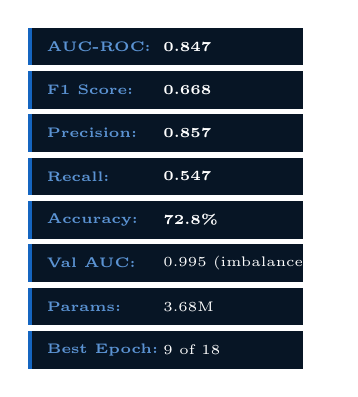
\begin{tikzpicture}
        \foreach \k/\v [count=\i] in {
          AUC-ROC/\textbf{0.847},
          F1 Score/\textbf{0.668},
          Precision/\textbf{0.857},
          Recall/\textbf{0.547},
          Accuracy/\textbf{72.8\%},
          Val AUC/0.995 (imbalanced),
          Params/3.68M,
          Best Epoch/9 of 18} {
          \fill[NavyBlue!50!black] (0,{-\i*0.55}) rectangle (3.5,{-\i*0.55+0.48});
          \fill[AccBlue] (0,{-\i*0.55}) rectangle (0.06,{-\i*0.55+0.48});
          \node[right, text=AccBlue!70!white, font=\tiny\bfseries] at (0.12,{-\i*0.55+0.24}) {\k:};
          \node[right, text=white, font=\tiny] at (1.6,{-\i*0.55+0.24}) {\v};
        }
      \end{tikzpicture}
    \end{column}
  \end{columns}
\end{frame}
}

\end{document}



\end{document}
